\section{Evolução e Manutenção de Software}

% Around 75\% of the maintenance effort was on adaptative or perfective changes, and error correction consumed about 21\%. \cite{bennett2000software}
% So software maintenance is important because (i) it consumes a large part of the overall lifecycle costs (ii) the inability to change software quickly and reliably means that business opportunities are lost. \cite{bennett2000software}

%%%%

A manutenção e evolução de software são atividades inevitáveis no trabalho com software - 
quase todo software útil e bem-sucedido estimula pedidos de mudança e melhorias gerados pelo usuário \cite{bennett2000software}. 
No entanto, a definição precisa dessas atividades ainda é objeto de debate.

O Instituto de Engenheiros Eletricistas e Eletrônicos (IEEE) define, em seu glossário, 
a manutenção de software como sendo a modificação de um produto de software após a entrega para 
corrigir falhas, melhorar desempenho ou outros atributos, ou adaptar o produto a um ambiente alterado. 
O IEEE ainda define os termos 'manutenção corretiva', 'manutenção adaptativa' e 'manutenção perfectiva', 
apontados na tipologia de manutenção de software de Swanson \cite{1990IEEESGo, swanson1976dimensions}.

\begin{itemize}
    \item Manutenção Adaptativa: realizada para tornar um programa de computador utilizável em um ambiente alterado;
    \item Manutenção Corretiva: realizada para corrigir falhas de hardware ou software;
    \item Manutenção Perfectiva: realizada para melhorar o desempenho, capacidade de manutenção ou outros atributos de um programa de computador.
\end{itemize}

Diversos pesquisadores adotaram a terminologia de Swanson, no entanto poucos utilizaram-na como foram 
definidas, o que causa confusão quanto a seu significado, uma vez que eles podem variar de acordo com 
quem a está usando. O próprio glossário do IEEE é parcialmente inconsistente com a definição original 
desses termos \cite{chapin2001types}. As três intenções para a manutenção de software 
apontadas por Swanson foram, em resumo:

\begin{itemize}
    \item Manutenção Adaptativa: para adaptar o sistema às mudanças no seu ambiente de dados ou ambiente de processamento
    \item Manutenção Corretiva: para corrigir falhas de processamento, desempenho ou implementação do sistema
    \item Manutenção Perfectiva: para aperfeiçoar o sistema em termos de desempenho, eficiência de processamento ou manutenibilidade
\end{itemize}

Chapin, por sua vez, define a manutenção de software como a aplicação proposital de atividades e 
processos, sejam eles completos ou não, em software existente, visando modificar a forma como o 
software dirige o hardware do sistema. Isso é geralmente realizado no contexto da evolução de software 
e difere da definição convencional encontrada no glossário do IEEE, uma vez que o status de 
'pós-implantação' ou 'após-entrega' para o software não faz parte da definição. 

Além disso, Chapin também define a evolução de software como a aplicação de atividades e 
processos de manutenção de software que geram uma nova versão de software operacional com uma funcionalidade 
ou propriedades experimentadas pelo cliente alteradas em relação à versão operacional anterior \cite{chapin2001types}. 
No entanto, assim como outros pesquisadores e profissionais, ele também utiliza o termo como sinônimo 
de manutenção de software, uma vez que o mesmo carece de uma definição padrão \cite{bennett2000software,chapin2001types}.

Em conjunto com essas definições, Chapin também propõem uma classificação objetiva e mais precisa dos 
tipos de atividades envolvidas na evolução e manutenção de software, com o objetivo de basear-se em 
evidências objetivas verificáveis através de observação e/ou comparação do antes e do depois do software; 
e de proporcionar uma classificação realista e prática para facilitar a comunicação e gestão da evolução 
e manutenção de software entre pesquisadores, profissionais e seus gestores \cite{chapin2001types}. 
A proposta de Chapin será detalhada de forma resumida na seção \ref{section:chapinTypes}.

\subsection{Classificação da evolução e manutenção de software proposta por Chapin}
\label{section:chapinTypes}

A classificação proposta por Chapin tem como base três critérios de decisão que se fundamentam sobre o 
local do sistema onde as atividades de manutenção ou evolução do software ocorrem, podendo essas serem 
realizadas no software (A), no código (B) ou nas funcionalidades experimentadas pelo cliente (C). 
Esses critérios são satisfeitos a partir da coleta de evidências objetivas, que são adquiridas 
por meio da comparação do software antes e depois das alterações.

A partir dos critérios atendidos, se define o \textit{cluster} ao qual essa atividade pertence, 
entre as quatro opções propostas e, por fim, são escolhidos os tipos de decisão, mutuamente exclusivos, 
condizentes com a atividade realizada, dentre as opções sugeridas no \textit{cluster} definido. 
Pode ser feita uma mistura ou agregação em qualquer ordem de alguns ou todos os tipos, mesmo que 
um tipo possa ser considerado ou observado como dominante.

A ordem dos tipos e seus clusters é significativa devido aos seus impactos diferentes, como ilustra 
a Fig. \ref{fig:impactOfTypes}. A dimensão horizontal representa o impacto da evolução ou manutenção na capacidade do 
usuário de utilizar o software de forma eficaz e na sua satisfação com o mesmo, da esquerda 
(baixo impacto) para a direita (alto impacto). O número de blocos sugere a faixa provável de impacto 
no cliente. A dimensão vertical representa o impacto da evolução ou manutenção no próprio software, 
de cima (impacto baixo) para baixo (impacto alto).

% \begin{figure}[h]
% 	\centering
%         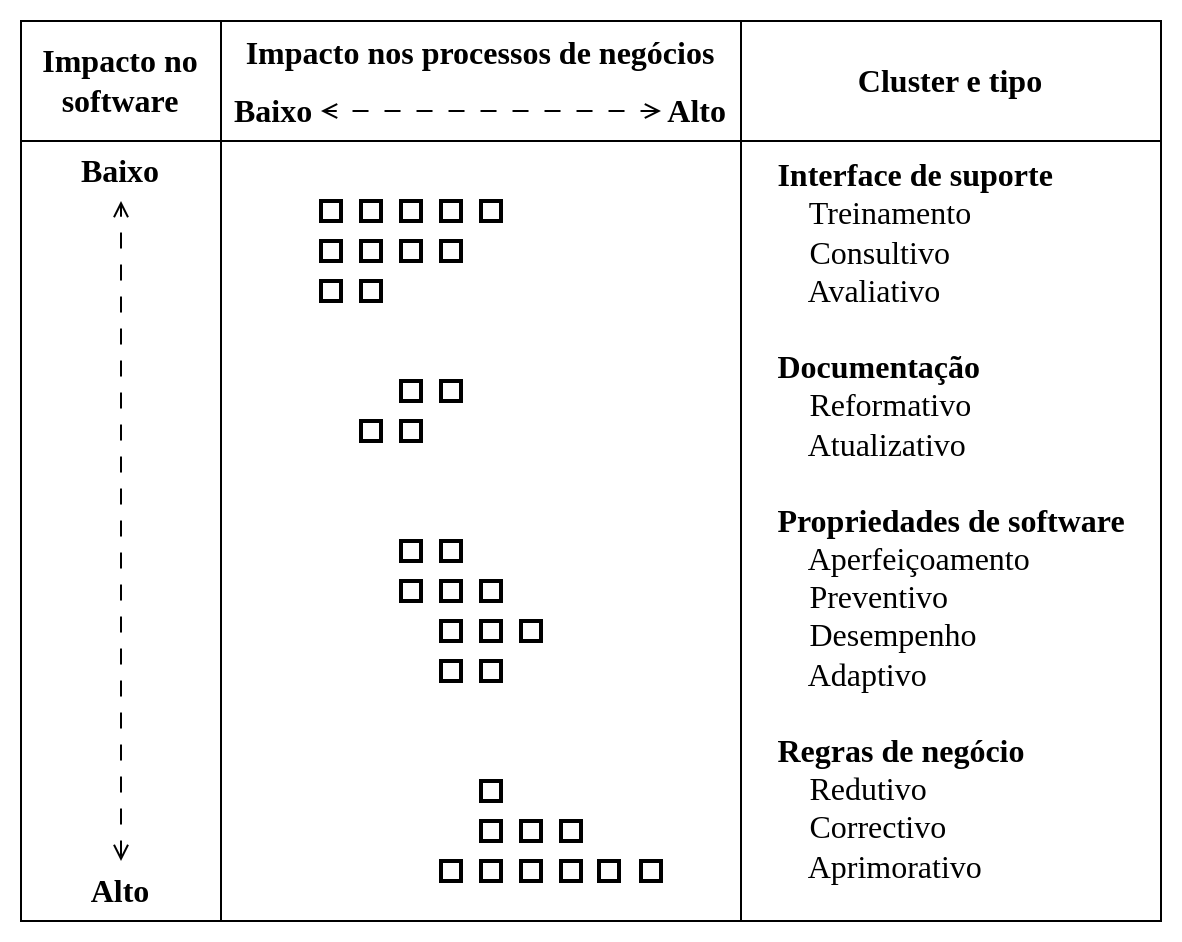
\includegraphics[keepaspectratio=true,scale=0.3]{figuras/evolutionMaintenance/impactOfTypes.png}
% 	\caption{Impacto dos tipos de evolução e manutenção de software.}
% 	\label{fig:impactOfTypes}
% \end{figure}

Para definição do tipo de evolução ou manutenção realizada, Chapin fornece uma árvore de decisão 
condensada, Fig. \ref{fig:decisionTreeForTypes}, com perguntas de 'Sim' ou 'Não' que encaminham para a opção mais apropriada. 
A analise é iniciada pela parte do sistema que sofreu alteração, A, B ou C, que indica o cluster 
adequado. Dentro de cada cluster são definidas perguntas para cada tipo, que são mostrados em itálico 
à sua direita, e só são aplicáveis quando a resposta associada aquela pergunta é "Sim". 

A leitura da árvore de decisão apresentada na Fig. \ref{fig:decisionTreeForTypes} deve ser realizada da esquerda para direita, 
enquanto os tipos devem ser lidos de baixo para cima, ambos levando em consideração os padrões de 
significância ilustrados na Fig. \ref{fig:impactOfTypes}, para que se obtenha um impacto crescente tanto no software 
quanto nos processos de negócios do cliente.

Dado que a evolução ou manutenção de software geralmente implica inúmeros processos ou atividades, a 
determinação do tipo requer a realização de várias perguntas na árvore de decisão. Progredir para a 
direita ou para cima na árvore de decisão deixa todos os tipos à esquerda e abaixo como candidatos ativos. 
E caso um tipo dominante não seja definido, a escolha padrão deve ser aquele com maior impacto que 
recebeu uma resposta positiva, ou seja, o "Sim" que estiver mais à direita e na posição mais alta.

O tipo de maior impacto dentro de um cluster também é a escolha padrão quando a evidência para 
discriminar entre os tipos está faltando ou é discutível. Por conta disso, também não é fornecido 
um tipo "Outro", já que, no caso de um evidência ambígua, existe um padrão a ser seguido.

Caso exista falta de evidências para definir os critérios de decisão A, B, e C, ou caso elas sejam 
discutíveis, a escolha padrão para responder a árvore de decisão deve ser "Não". Por fim, se a 
observação e outras evidências indicarem que não foram realizadas atividades ou processos além 
dos relacionados à execução do software, não houve ocorrência de evolução ou manutenção de software.

% \begin{landscape}
%     \begin{figure}[h]
%     	\centering
%     	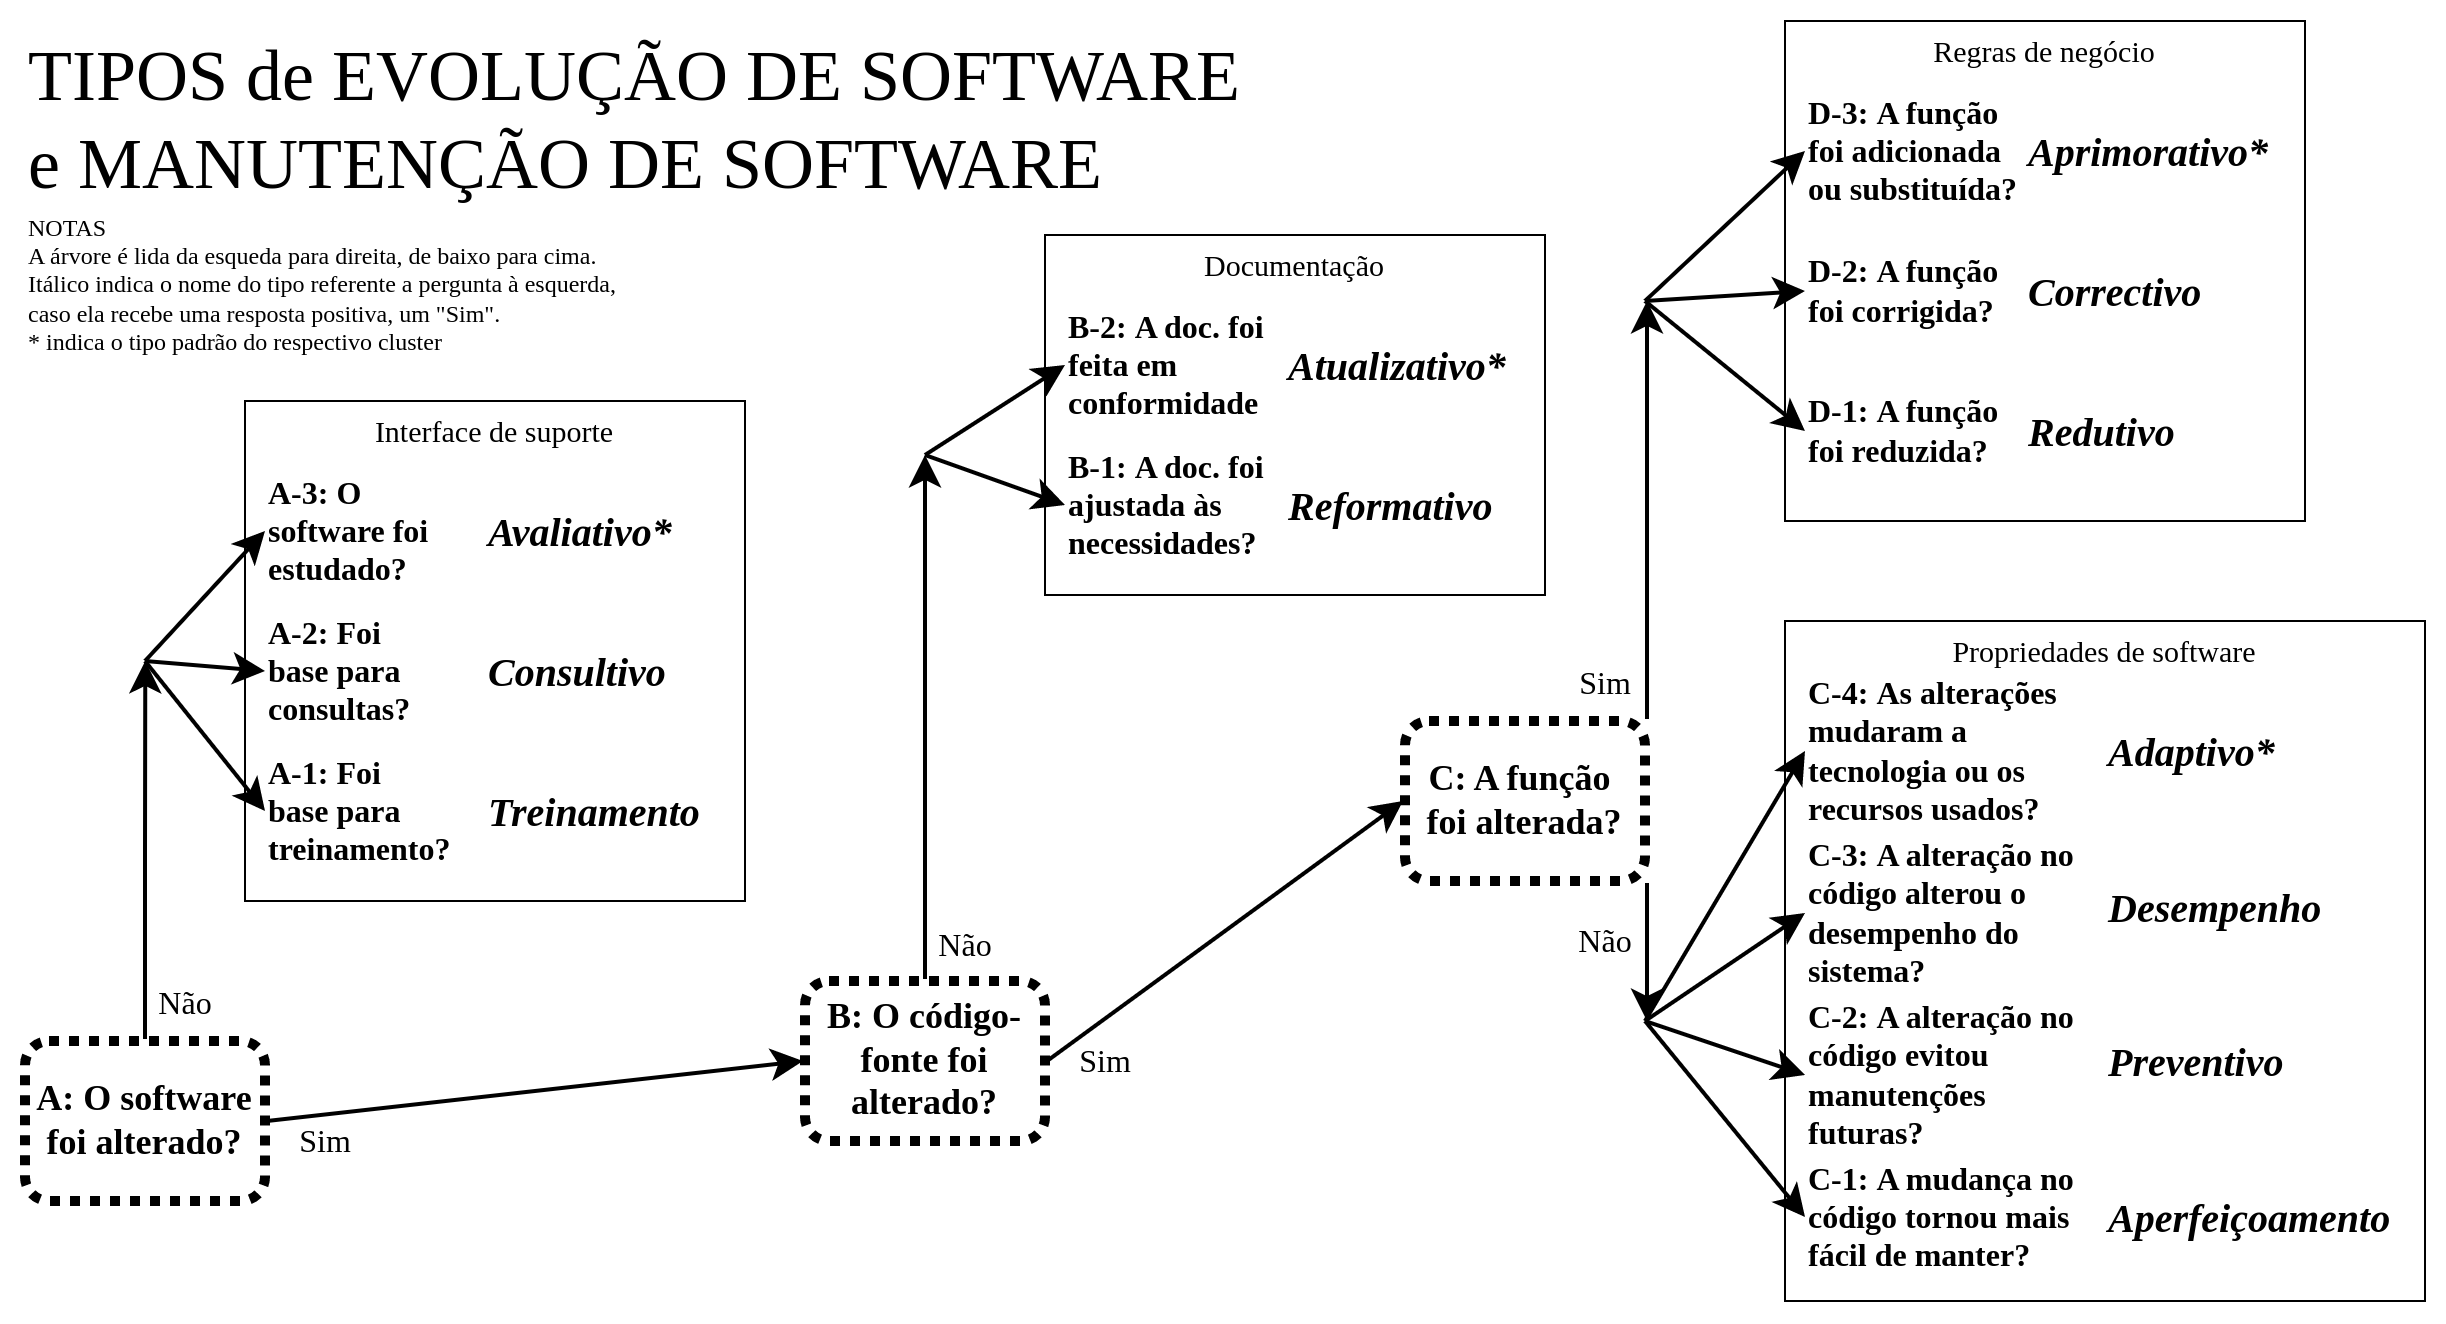
\includegraphics[keepaspectratio=true,scale=0.25]{figuras/evolutionMaintenance/decisionTreeForTypes.png}
%     	\caption{Árvore de decisão para os tipos.}
%     	\label{fig:decisionTreeForTypes}
%     \end{figure}
% \end{landscape}

Diante da ampla variedade de atividades executadas no âmbito da evolução e manutenção de software, 
é possível observar uma variedade de tipos, mesmo quando um tipo particular é predominante. A Fig. \ref{fig:relationAmongTypes} 
ilustra de maneira simples a relação encontrada entre os tipos definidos, onde os superiores são mais 
significativos porque têm mais impacto no cliente ou no software ou em ambos.

A chave para entender essa relação retoma os três critérios de decisão A, B e C. Responder 
"Não" para um desses critérios identifica de imediato um \textit{cluster} respectivo, onde terá 
pelo menos um tipo de decisão que será escolhido. No entanto, ao responder com "Não" um critério 
mais impactante, ou seja, que esteja mais a direita, também corresponde a responder com "Não" os 
critérios menos impactantes, adicionando os respectivos \textit{clustes} à analise. 

Apesar da explicação ser complicada, na prática, ao selecionar um tipo de evolução ou manuntenção 
de software, todos os tipos que estiverem listados abaixo dele na Fig. \ref{fig:relationAmongTypes} também serão observados 
durante a realização das atividades, mesmo quem em pequena quantidade.

% \begin{figure}[h]
% 	\centering
% 	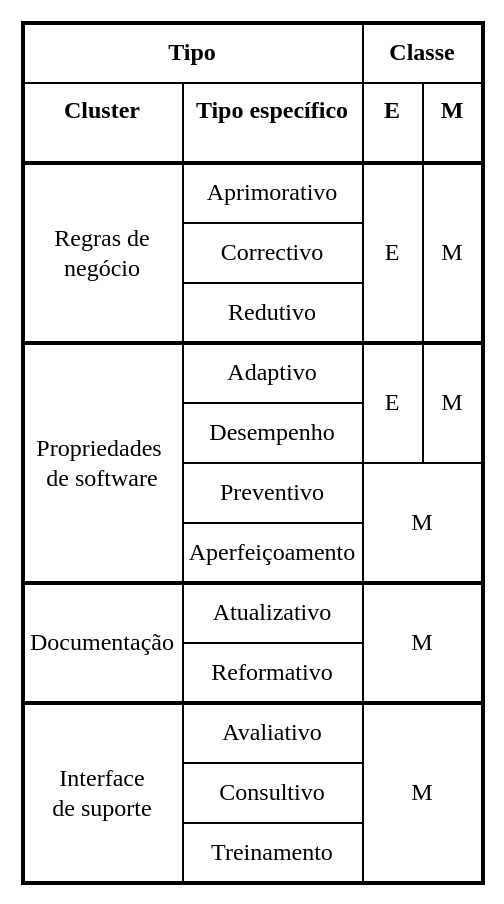
\includegraphics[keepaspectratio=true,scale=0.3]{figuras/evolutionMaintenance/relationAmongTypes.png}
% 	\caption{Relação entre os tipos, onde E indica evolução de software, e M indica manutenção de software.}
% 	\label{fig:relationAmongTypes}
% \end{figure}

% Isso entraria como apêndice?
Os tipos de evolução e manutenção de software propostos por Chapin são definidos como:

\begin{itemize}
    \item Cluster de interface de suporte
    \begin{itemize}
        \item Treinamento (\textit{Training}): envolve atividades como ministrar aulas para o pessoal do cliente, 
        realizar treinamentos, on-site na empresa do cliente ou ambulantes, e utilizar materiais de 
        treinamento existentes;
        \item Consultivo (\textit{Consultive}): envolve atividades como atender perguntas sobre o software em uma central 
        de ajuda para o pessoal do cliente, discutir com o pessoal ou gerentes do cliente sobre o uso 
        eficaz de um sistema ou sobre a realização de (propostas ou possíveis) alterações no software, 
        e aconselhar clientes, gerentes ou outros interessados (ou mesmo pesquisadores) sobre o tempo, 
        custo, atividades ou esforço necessários para realizar trabalhos de evolução ou manutenção 
        solicitados ou contemplados.
        \item Avaliativo (\textit{Evaluative}): envolve atividades como auditoria, busca, examinação, teste de regressão, 
        estudo, teste diagnóstico, fornecimento de ambientes de teste protegidos, cálculo de métricas 
        sobre, ou criação de uma compreensão do software sem alterá-lo.
    \end{itemize}
    \item Cluster de Documentação
    \begin{itemize}
        \item Reformativo (\textit{Reformative}): altera a forma da documentação não-código, sem alterar o código. Isso inclui 
        atividades como alterar o formato ou cobertura de um manual do usuário.
        \item Atualizativo (\textit{Updative}): envolve atualizar, polir e aumentar a cobertura de documentação não-código, 
        como substituir documentação não-código obsoleta por documentação atual ou preencher lacunas na 
        documentação não-código, incluindo planos de teste, visões gerais narrativas, modelos UML, etc., 
        sem alterar o código.
    \end{itemize}
    \item Cluster de propriedades de software
    \begin{itemize}
        \item Aperfeiçoamento (\textit{Groomative}): envolve atividades de cuidado com o código fonte, como recompilações, 
        substituição de componentes ou algoritmos por outros mais elegantes, criação de backups de 
        código, alteração de autorizações de acesso pessoais ou de nível, alteração de comentários ou 
        linhas de anotação de código fonte, alteração de convenções de nomenclatura de dados, alteração 
        da legibilidade ou compreensibilidade do código e fornecimento de mensagens de erro menos crípticas.
        \item Preventivo (\textit{Preventive}): envolve alterações que não afetam as funcionalidades experimentada pelo cliente 
        ou a tecnologia ou recursos utilizados. Os resultados dessas atividades preventivas raramente 
        são diretamente perceptíveis pelo cliente.
        \item Desempenho (\textit{Performance}): envolve processos como a redução do uso de armazenamento interno, melhoria do 
        tempo de atividade do sistema, redução da duração de períodos fora de serviço, aumento da 
        velocidade de execução, substituição de componentes ou algoritmos por outros mais rápidos e 
        melhoria da confiabilidade e robustez do sistema. A mudança em tais propriedades geralmente é 
        percebível pelo cliente.
        \item Adaptivo (\textit{Adaptive}): envolve processos como adaptar o sistema para funcionar em uma plataforma 
        diferente, com um sistema operacional modificado ou com um tipo diferente de banco de dados, 
        redistribuir as funções entre componentes ou sub-sistemas, aumentar a utilização de COTS, 
        alterar os protocolos de comunicação suportados, mudar a interoperabilidade do sistema e mudar 
        práticas de design e implementação.
    \end{itemize}
    \item Cluster de regras de negócio
    \begin{itemize}
        \item Redutivo (\textit{Reductive}): de particular importância para a evolução de software, envolve limitar ou 
        eliminar algumas regras de negócios do repertório implementado, como substituir, restringir 
        ou remover parte ou todos os componentes, algoritmos ou sub-sistemas. Fluxos de dados podem ser 
        eliminados ou reduzidos.
        \item Correctivo (\textit{Corrective}): envolve aprimorar e especificar a implementação das regras de negócios 
        existentes para lidar melhor com exceções e casos mal gerenciados, geralmente adicionando 
        precisão adicional à lógica interna de alguns componentes, algoritmos ou sub-sistemas, ou 
        adicionando mais programação defensiva. Este tipo costuma ser reativo, para remoção de defeitos 
        ('bugs') como aqueles originados de falhas de design ou erros de codificação.
        \item Aprimorativo (\textit{Enhancive}): é particularmente significativo para a evolução de software, pois implementa 
        mudanças e adições ao repertório de regras de negócios implementadas pelo sistema, inserindo 
        novos componentes, algoritmos ou sub-sistemas e alterando os existentes para ampliar ou estender 
        seu escopo. Novos fluxos de dados podem ser adicionados e os fluxos de dados existentes podem 
        ser redirecionados.
    \end{itemize}
\end{itemize}
